\documentclass[]{article}
\usepackage[utf8]{inputenc}
\usepackage{fullpage}
\usepackage{listings}
\usepackage{graphicx}

\title{CS 526 Information Security \\\textbf{Project 2 - Software Security}}

\date{Due Nov 28th, 2012}

\begin{document}
\newcommand{\comment}[1]{}

\maketitle

In this project, you will perform a series of software vulnerability
exploits. You will explore unsafe and insecure programming techniques
and will evaluate the efficacy of operating system defenses against
them.

\section*{Instructions}

\paragraph{Due date \& time} 11:59pm on Nov 28th, 2012. Email your
report to the TA (gates2@purdue.edu) by the due time.


\paragraph{Late Policy} You have three extra days in total for all
your homework and projects. Any portion of a day used counts as one
day; that is, you have to use integer number of late days each
time. If you emailed your homework to the TA by 11:59pm the day after
it is due, then you have used one extra day. If you exhaust your three
late days, any late project won’t be graded. 

\paragraph{Additional Instructions}

\begin{itemize}
\item You will work on this project individually.
\item For this project, you will need to access a virtual machine that is set up on \verb"forest.cs.purdue.edu". Each student will use their account from the last project on \verb"forest.cs.purdue.edu".
\item You will use another username/password to access the virtual machine, you should have already received an email with this information. After logging into \verb"forest", you can access the virtual machine via ssh:\\ \verb"ssh attackme"
\item The source files you need can be found in your home directory. The targets will be in a tar archive in the directory \verb"~/targets/". 
\item The source code of your answers needs to be in the directory \verb"~/exploits/" by the deadline. You need to hardcode relative paths in your source code to execute the targets.
\item Any code you write should run on the virtual machine in forest with no errors.
\item The written portion of the project must be typed. Using Latex is recommended, but not required. The submitted document must be a PDF (no doc or docx are allowed)
\item Most of the points for each question will be for a correct exploit. If you answer a question without correctly exploiting the target, no credit will be given.
\item You are NOT allowed to modify the source code for any of the targets.
\end{itemize}

\newpage 

\section{(15 pts) Get the Code}

The files needed to complete the project are in an archive called
\verb"project2_files.tar" in your home directory. This archive,
however, is encrypted. Only one user (username = \verb"poorvictim")
knows the decryption key. The key is stored in \verb"poorvictim"'s
home directory. However, all the access control bits are set such that
only \verb"poorvictim" can read the file.

In order to help CS 526 students, \verb"poorvictim" has created a
program that can read the secret in the file. This program is owned by
\verb"poorvictim" and has the setuid bit set; thus, it can run with
\verb"poorvictim"'s privileges. The program is available to all
students and can be found in the following path:\\

\verb"/usr/bin/getcode"

In order to make life harder for CS 526 students, \verb"poorvictim"
made \verb"getcode" require a password as a command line argument
before releasing the key. The first 3 characters of this password need
to adhere to some strange mathematical property. However, no one knows
how to create a password that satisfies this requirement! Fortunately,
the program has an obvious buffer overflow vulnerability.


In this section, you will exploit a buffer overflow vulnerability in a
program that has the setuid bit set. This will help you get the
password to decrypt the files needed to complete the rest of the
project. Your goal is to pass a password to \verb"getcode" and make it
accept the password.  The successful exploitation will make the
program print:

\begin{verbatim}
	Access granted to the document ...
\end{verbatim}
followed by the decryption key.

\begin{itemize}
\item In the exploits directory, write a shell script
  \verb"exploit1.sh" that passes the attack string to the target and
  performs the attack. You do not have access to the target's source
  code. Thus, you will have to use \verb"gdb" to disassemble the
  program. A good place to start is the \verb"main" function.

\item Identify the exact vulnerability in the program that you
  exploited (i.e. function name)
  \begin{itemize}
  \item   The vulnerability I exploited was in the strcpy function
    inside of main(line 54) and the fact it doesn't check the length
    of the input entered by the user to make sure it will fit inside
    the 16 byte buffer into which it is copying.
  \end{itemize}
  
\item Explain your attack strategy. Include in your answer an
  explanation for how you determined the crafted password.\\

  \begin{itemize}
  \item 
    My attack strategy is to overflow the buffer allocated for the
    \emph{passwd} variable and thus write into the \emph{decision}
    variable. From examining the assembly we can see that there are 28
    bytes in between the start of \emph{passwd} and the start of
    \emph{decision}. This can be determined with the assembly lines of:
    \begin{lstlisting}
      0x8048725 <main+61>:mov    %eax,0xfffffff4(%ebp)
      0x8048733 <main+75>:lea    0xffffffd8(%ebp),%eax
    \end{lstlisting}
    These two lines show the start locations of \emph{decision} and
    \emph{passwd} (relative to \%ebp). From this we know that a string
    of length 29 is needed to overflow \emph{passwd} into
    \emph{decision}. Once \emph{decision} is written into the final
    check to see if the correct password was entered will always succeed. 
  \end{itemize}
  
\item Assuming an attacker can always find a vulnerability to exploit
  to bypass the password check. What can \verb"poorvictim" do to
  always prevent the leakage of information if the password is
  incorrect?
  \begin{itemize}
  \item \verb"poorvictim" could encrypt the password inside
    secret.txt. Then when getcode executes it will use the password
    entered to decrypt the file. In this way even if the attacker is
    able to bypass the password check it will not decrypt the file
    properly therefore producing the wrong password.
  \end{itemize}
  
\item Give the decryption string that you recovered in your report.\\
  \begin{itemize}
  \item "TheB3St1337P@\$\$w0rd"
  \end{itemize}
\end{itemize}

Use the decryption key to decrypt the archive by running the following command:\\
\verb"gpg project2_files.tar.gpg"
After recovering the source files, run \verb"make" to compile the rest
of the targets

\section{(25 pts) Buffer Overflow}

In this section, you will exploit buffer overflow vulnerabilities in
poorly written programs.  

\begin{enumerate}

\item \verb"target2" is a program that takes a directory as input, and
  tells the user how to use the command \verb"ls" to list the contents
  of the directory. Suppose that this program is setuid root. You will
  login as a normal user, and your goal is to pass an argument to the
  program so it will start a root shell.
  
  \begin{itemize}
  \item In the exploits directory, write a shell script
    \verb"exploit2.sh" that passes the attack string to the target and
    performs the attack. 
  \item Identify the exact vulnerability in the program that you
    exploited (i.e. function name and line number) 
    \begin{itemize}
    \item The vulnerability I exploited was in the call to system on
      line 21. 
    \end{itemize}
  \item Explain your attack strategy. That is, explain how you
    determined the correct input to pass and what commands are
    executed.
    \begin{itemize}
    \item The strategy used in this attack was simply to execute
      multiple commands in the call to system. This is accomplished by
      ending the first command with a semicolon and executing a
      command to launch a shell (e.g. /bin/sh). The is done with the
      string "; /bin/sh". First, system will execute "ls --color -l ;"
      and then it will execute "/bin/sh".
    \end{itemize}
  \end{itemize}
  
\item \verb"target3" is a program that takes a customer's name as the
  input, and prints a coupon.  Assume that each customer can only
  execute the program once, so he/she can only get one coupon.  Your
  goal is to pass some argument to the program so it will repeatedly
  print coupons.  In other words, the argument will make the program
  execute the function {\em coupon} repeatedly. Note: To get full
  credit, the function \verb"coupon" has to execute an \emph{infinite}
  number of times. If it only executes twice, then you will get half
  the points.
    
  \begin{itemize}
  \item In the exploits directory, write a C program \verb"exploit3.c"
    that passes the attack string to the target and performs the
    attack.
  \item Identify the specific bug/vulnerability that made your attack
    possible.\\
    \begin{itemize}
    \item 
      The bug that makes this attack possible is in the blind string
      copy from the input string into the local variable \emph{name}. We
      can see that name is initialized to 16 bytes of data but the size
      of the string used for input is not restricted or checked to make
      sure it is less than 16 bytes. 
    \end{itemize}
  \item Describe your attack strategy. That is, describe the memory
    addresses involved in your attack, and explain how the attack made
    the program print an unlimited number of coupons.\\
    \begin{itemize}
    \item The strategy used in this attack was to overwrite the ebp
      value on the stack with the correct ebp value for the function
      main() and overwrite the return address to return back to the
      location prior to the call to coupon that would place the
      arguments back on the stack and call coupon again. The ebp value
      discovered for main was: 0xbffffeb8 and the address returned to
      was: 0x8048619. To make the attack more stable environmental
      variables are cleared prior to executing the target, which is
      launched via execv(). The address for the ebp register was
      determined using inline assembly inside of the main function and
      the return address was determined using gdb. The reason this
      attack will continue on an infinite number of times is because
      it is, in essence, recalling coupon an infinite number of
      times. Almost as if coupon had been placed inside a
      non-terminating loop.
    \end{itemize}
  \end{itemize}
  
\item The machine \verb"forest" has an updated operating system with
  some stack defenses activated.
  \begin{itemize}
  \item Repeat the attack on \verb"target3" outside the virtual
    machine. Did the attack work? Comment on your results
    (i.e. explain why)\\

    \begin{itemize}
    \item The attack did not work, failing on with the error:\\
\begin{verbatim}
  *** stack smashing detected ***: ../targets/target3 terminated
\end{verbatim}
What's happened here is that gcc has included canary values
(i.e. random values) into the
stack to detect when this type of attack is being performed. These
values are generally inserted between the ebp value on the stack and
the local variables. This way when the canary value is overwritten
it's clear the behavior of the program is not that of the intended behavior.
    \end{itemize}
  \item Propose \textbf{two} different operating system and/or
    compiler/programming language defenses that can be used to prevent
    this attack from working. Discuss the advantages, disadvantages,
    and feasibility of the proposed defenses. 
    
    \begin{enumerate}
    \item Address space layout randomization: In this defense all the
      addresses will be randomized when the program is executed. This
      will help prevent against this kind of attack because the return
      address and ebp values we've used in the attack would be
      different for every execution of the target. The disadvantage
      to this type of defense is that there is overhead involved in
      randomizing address with each execution and this is something
      that must be supported in the OS kernel. However, this is fairly
      common in modern kernels thus making the defense feasible in
      modern systems.
    \item Bounds checking for arrays: This defense will help us by
      alerting the system that an array access has exceeding the
      memory allocated for that array. In this instance we will detect
      that we have attempted to copy more than the 16 bytes allocated
      for name and the program can be terminated. Bounds checking
      comes with a decrease in performance naturally. This is because
      with each access to an array element the system must check to
      make sure that access is within the memory allocated for that
      array. This type of checking is generally not implemented in C
      so if one wanted to use this as a defense they would need to
      write code in a different language. 
    \end{enumerate}
  \end{itemize}
\end{enumerate}

\section{(20 pts) The Dangers of the Executable Stack}

\begin{enumerate}
\item \textbf{The attack}: \verb"target4" is a program that takes a
  user's password as the input, and checks if the password is a
  `strong' one or a `weak' one 
  Assume that \verb"target4" is setuid root.  You will login as a
  normal user, and your goal is to pass an argument to the program to
  start a root shell. The shellcode is provided in {
    \verb"/home/user/exploits/shellcode.h"}. 

  \begin{itemize}
  \item In the exploits directory, write a C program \verb"exploit4.c"
    that performs the attack. 
  \item Identify the specific bug in the program and vulnerability in
    the operating system that made your attack possible.
    \begin{itemize}
    \item The bug in the program that made this possible was the
      string copy from arg into password without a length check on the
      input argument.
    \end{itemize}
  \item Describe your attack strategy. That is, explain what memory
    addresses you used and how you figured out those addresses.
    \begin{itemize}
    \item The attack strategy for this exploit was to fill part of the
      passwd buffer with the provided shell code and overwrite the
      return address to return the beginning of that shell code in
      order to execute the shell. The addresses I discovered to return
      to was 0xbffffe20, which is the address of passwd. This was
      discovered by setting up the attack string and launching the
      target from the exploit with environmental variables
      cleared. The offset found for passwd was found to be 72 bytes
      (from ebp) and was discovered using gdb. 
    \end{itemize}
  \item Draw the layout of the stack frame corresponding to the
    function \verb"check" directly after the local variables are
    initialized. For each element on the stack, provide its size
    (assuming a 32-bit architecture).
    \begin{figure}[h!]
      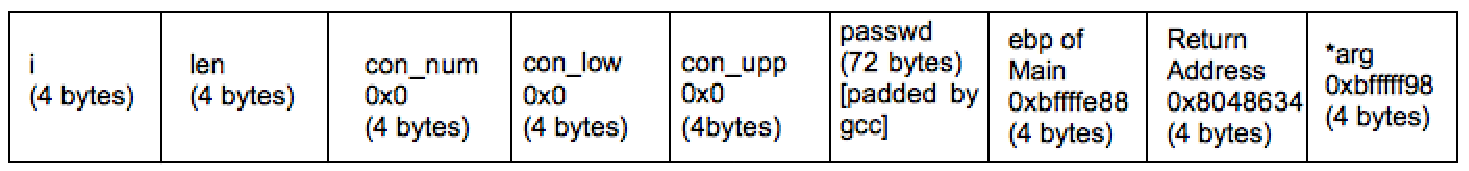
\includegraphics[width=\textwidth]{images/stack3_0.pdf}
      \caption{Stack prior to exploit.}
    \end{figure}
  \item Draw the layout of the stack frame corresponding to the
    function \verb"check" directly after the vulnerable statement
    executes with your injected code (i.e. how it looks after the
    overflow). How do the values you injected influence the control
    flow of the program?
    \begin{itemize}
    \item The values I've injected into the stack influence the
      control flow in one critical way: they overwrite the return
      address of \emph{check()} such that it will return to a location
      of my choice. In this exploit the address I have returned to is
      that of the variable \emph{passwd} which, after my attack,
      contains the code necessary to execute a shell.
    \end{itemize}
    \begin{figure}[h!]
      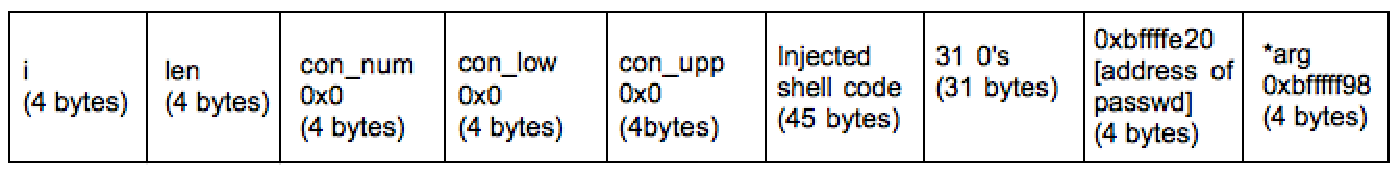
\includegraphics[width=\textwidth]{images/stack3_1.pdf}
      \caption{Stack after the exploit.}
    \end{figure}
  \end{itemize}
  
  
\item \textbf{The defense}: Try repeating the above attack on
  \verb"forest" (outside the virtual machine).  
  \begin{itemize}
  \item Are you able to get the attack to work? 
  \item What specific mechanism(s) make the attack more difficult?
    \begin{itemize}
    \item On \verb"forest" I am unable to get the attack to
      work. There are two mechanisms preventing this from functioning
      on forest. The first of which is the canary values inserted into
      the stack by gcc. With these enable an error such as seen
      previously is reported:
      \begin{verbatim}
        *** stack smashing detected ***: ../targets/target4 terminated
      \end{verbatim}
      This, however, can be disabled in gcc with the
      -fno-stack-protector flag. However, even with this disabled the
      OS on \verb"forest" has enabled address space layout
      randomization so obtaining the address of \emph{passwd} to set
      the return address becomes very very difficult.
    \end{itemize}
  \end{itemize}
\end{enumerate}

\section{(20 pts) Return to libc} 

\begin{enumerate}
\item \textbf{The attack}: \verb"target5" is a program that scans several network packets and checks if the traffic (concatenation of the packets) matches any virus signatures. Suppose \verb"target5" is setuid root. You will login as a normal user, and the goal is to pass argument(s) to the program to start a root shell. You need to assume that the stack is \textbf{not} executable. Therefore, you \textbf{cannot} change the return address to the shellcode in the stack.
  
  \begin{itemize}
  \item Draw the layout of the stack frame corresponding to the
    function \verb"is_virus" directly after the local variables are
    initialized. For each element on the stack, provide its size
    (assuming a 32-bit architecture).
    \begin{figure}[h!]
      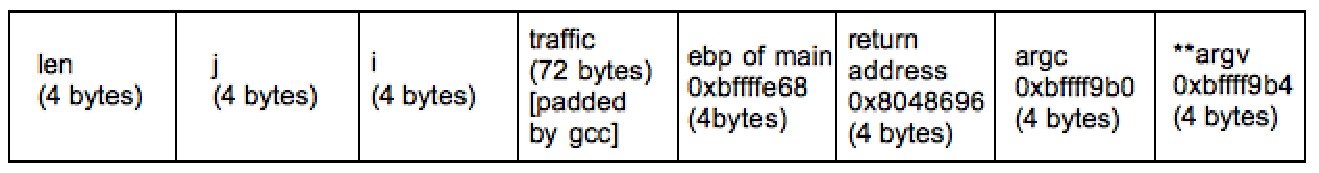
\includegraphics[width=\textwidth]{images/stack4_0.pdf}
      \caption{Stack prior to return-to-libc exploit.}
    \end{figure}
  \item In the exploits directory, write a C program \verb"exploit5.c"
    that performs the attack.
  \item Identify the specific bug in the program and vulnerability in
    the operating system that made your attack possible.
    \begin{itemize}
    \item The specific bug used in this exploit was that there is no
      check on the amount of characters that are concatenated to the
      end of \emph{traffic}. This variable is initialized to 64 bytes
      and the input that the user enters is blindly concatenated into
      this buffer with no check to make sure the user hasn't entered
      more than 64 bytes.
    \end{itemize}
  \item Describe your attack strategy. That is, explain what memory
    addresses you used and how you figured out those addresses.
    \begin{itemize}
    \item The strategy used in this exploit was to modify the return
      address of \emph{is\_virus()} to be that of the \emph{system()}
      function with a parameter of "/bin/sh". To accomplish this I
      introduced an environmental variable called \emph{myshell} which
      contained the string "/bin/sh" and added the address of this
      onto the stack for the parameter to system. The attack string
      consists of 76 bytes of junk (the offset between traffic and the
      return address) followed by the address of system (0x80483d4,
      discovered via printf() inside of target5), followed by 4 bytes
      of junk, followed by the address of the myshell variable
      (0xbfffffe1, discovered via getenv() inside of target5).
    \end{itemize}
  \end{itemize}
  
\item \textbf{The defense}: Try repeating the above attack on
  \verb"forest" (outside the virtual machine). The attack should
  become more difficult now.
  \begin{itemize}
  \item Are you able to get the attack to work? If so, explain your
    method. Otherwise, explain what prevented you from completing the
    attack.
  \item What specific mechanism(s) make the attack more difficult?
    \begin{itemize}
    \item Once again this attack was unable to be reproduced on
      \verb"forest". If the target is compiled with stack protection
      we once again see the error:
      \begin{verbatim}
        *** stack smashing detected ***: ../targets/target5 terminated
      \end{verbatim}
      However, there is also address space layout randomization being
      used. This means that the address of system() and myshell will
      be randomized with each execution of the program thus making the
      attack much more difficult to perform.
    \end{itemize}
  \end{itemize} 
\end{enumerate}

\section{(20 pts) Format String Attacks}

In this section, you are given a program with a format-string
vulnerability; your task is to develop a scheme to exploit the
vulnerability. You can find the source code for the program is
\verb"target6.c". 

In \verb"target6.c", you will be asked to provide an input, which will
be saved in a buffer called {\tt user\_input}. The program then prints
out the buffer using {\tt printf}. Unfortunately, there is a
format-string vulnerability in the way the {\tt printf} is called on
the user inputs. We want to exploit this vulnerability and see how
much damage we can achieve. 

The program has two secret values stored in its memory, and you are
interested in these secret values. However, the secret values are
unknown to you, nor can you find them from reading the  binary code
(for the sake of simplicity, we hardcode the secrets  using constants
0x$44$ and 0x$55$, but you can pretend that you don't have the source
code or the secrets).  Although you do not know the secret values, in
practice,  it is not so difficult to find out  the memory address (the
range or the exact value) of them (they are  in consecutive
addresses), because for many operating systems, the addresses are
exactly the same anytime you run the program.  

\begin{itemize} 
\item Draw the layout of the stack frame corresponding to the main
  function directly after the local variables are initialized. For
  each element on the stack, provide its size (assuming a 32bit
  architecture). 
  
\item Provide the specific inputs (i.e. both the integer and the
  string) that you need in order to crash the program. Explain why the
  program crashes with your input.
  \begin{itemize}
  \item integer: 5 string:
    \%p$|$\%p$|$\%p$|$\%p$|$\%p$|$\%p$|$\%p$|$\%p$|$\%p$|$\%p$|$\%p$|$\%s
  \item The reason this crashes is that I am trying to print from the
    memory address located on the stack right above secret. This value
    is going to be an undefined memory location since it corresponds
    to memory reserved for \emph{user\_input} and is therefore the
    first four bytes of the string I entered. In this case \%p$|$ or
    0x7c7c7025. When the \%s at the end of the input string tries to
    read from this memory location the program crashes with a
    segmentation fault because this is not a valid area of memory to
    be read from.
  \end{itemize}
  
\item Provide the specific inputs (i.e. both the integer and the
  string) that you need in order to print the \emph{address} of the
  variable \verb"secret[0]". Explain why you think this is the correct
  address. Hint: you can use \verb"gdb" to verify that your answer is
  correct.\\
  \begin{itemize}
  \item integer: 5. string:
    \%p$\|$\%p$\|$\%p$\|$\%p$\|$\%p$\|$\%p$\|$\%p$\|$\%p$\|$\%p$\|$\%p$\|$\%p\\
    The output:\\
    0xbffff960$\|$0x400212b8$\|$0xbffff97c$\|$0x4002c8a4$\|$0x40021000$\|$0x400212d8$\|$0x1$\|$(nil)$\|$(nil)$\|$0x5$\|$0x8049818\\
    The reason I believe this to be the correct value is because from
    looking at the code we can see that the variable \emph{int\_value}
    is declared right after the variable \emph{*secret}. This means
    that, on the stack, \emph{*secret} should appear directly after
    \emph{int\_value}. Since I've put the value of 5 into
    \emph{int\_value} it stands to reason the next value printed would
    be the pointer to secret. This is confirmed in gdb by breaking
    somewhere in main and printing secret to obtains it address.
  \end{itemize}
  
\item Provide the specific inputs (i.e. both the integer and the
  string) that you need in order to print the \emph{value} of
  \verb"secret[0]". Explain your strategy.
  \begin{itemize}
  \item integer: 5 string: \%11\$s. The strategy used here is that
    from the previous examples we can see that the address for
    secret[0] is the 11th element printed. We therefore construct the
    string that prints what is in the address located at the 11th
    element on the stack. 
  \end{itemize}
  
\item Based on your knowledge of how arrays are stored on the heap,
  calculate the address of \verb"secret[1]".
  \begin{itemize}
  \item On this system ints are stored as 4 bytes. This means that in
    the heap \verb"secret[1]" will be placed 4 bytes higher than
    \verb"secret[0]". In this instance at 0x804981c.
  \end{itemize}
  
\item Provide the specific inputs (i.e. both the integer and the
  string) that you need in order to print the value of
  \verb"secret[1]". Explain your strategy.
  \begin{itemize}
  \item integer: 134518812 string: \%10\$s. This is the same idea as
    that of printing secret[0] with the only difference being we
    inject the integer value of the address of secret[1] into
    \emph{int\_input} then we print what is in memory at that
    location. Previously we saw that \emph{int\_input} is located at
    the 10th element on the stack so we print what is in memory
    corresponding to the 10th element.
  \end{itemize}
\item Provide the specific inputs (i.e. both the integer and the
  string) that you need in order to modify the values of \emph{both}
  \verb"secret[0]" AND \verb"secret[1]". Explain your strategy.
  \begin{itemize}
  \item integer: 134518812 string: \%6.2s\%11\$n\%5.2s\%10\$n. In this
    example I am writing 6 to secret[0] and 11 to secret[1]. The
    strategy is, just like reading from secret[0] and secret[1], to
    utilize the knowledge that we know their offsets into the
    stack. So, in this attack I write 6 bytes then with \%11\$n I put
    the number of bytes into the memory location pointed to by the
    11th offset into the stack (i.e. secret[0]) then I write 5 more
    bytes and put this into the address located at the 10th offset
    into the stack (i.e. int\_input = secret[1]).
  \end{itemize}
\item Does address space randomization make this attack more
  difficult? Explain.
  \begin{itemize}
  \item ASR will make writing to secret[1] harder in this attack. The
    reason for this is the address of secret[0] will always be on the
    stack so even if it is random we will still be able to access it via
    the methods previously described for this attack. However, in this
    attack we have been computing the address of secret[1] in
    reference to secret[0] and using that as the method for accessing
    that address. If the address of secret is randomized with each
    execution this method will no longer be viable and will make that
    part of that attack more difficult.
  \end{itemize}
\item What other operating system defenses can be used to prevent this
  attack? Explain.
  \begin{itemize}
  \item The main operating system defense that could be used to
    prevent this type of attack is ensuring that functions only access
    memory locations inside their current stack frame. This will
    prevent the \emph{printf()} function from reading memory locations
    that are outside it's frame of reference. Another possible defense
    against this is to warn the programmer, at compile time, if they
    are using potentially harmful variables inside of printf
    statements. These variables could be found by the fact that they
    rely on user input.
  \end{itemize}
\end{itemize} 


\bibliographystyle{plain}
\bibliography{}
\end{document}
